% !TEX options=-shell-escape
\documentclass[12pt]{article}
\usepackage{amsfonts}
\usepackage{amsmath}
\usepackage{siunitx}
\usepackage{fancyvrb}
\usepackage{hyperref}
\usepackage{makecell}
\usepackage[a4paper, total={7in, 10in}]{geometry}
\usepackage{tikz}
\usepackage{footnote}
\usepackage{subcaption}
\usepackage{graphicx}
\usepackage{libertine}
\usepackage{minted}
\usepackage[nottoc]{tocbibind}
\usepackage{tablefootnote}
\usepackage{xeCJK}
\usepackage{soul}
\usepackage{datetime}

\newdateformat{chinesedate}{\THEYEAR 年\THEMONTH 月\THEDAY 日}

\makesavenoteenv{tabular}
\makesavenoteenv{table}

\definecolor{bg}{rgb}{0.95,0.95,0.95}
\setminted{
  fontsize=\footnotesize,
  bgcolor=bg,
  frame=leftline
}

\providecommand{\keywords}[1]{\small\textbf{\textit{Keywords---}} #1}

\date{Friday $11^\text{th}$ September, 2020}

\title{A multifunctional hamiltonian mechanics simulator and some of its application examples}
\author{詹有丘 (Youqiu Zhan)}

\begin{document}

\Huge

~\par
~\par
\noindent 参赛队员姓名:\underline{詹有丘}\par
~\par
\noindent 中学:\underline{上海交通大学附属中学}\par
~\par
\noindent 省份:\underline{上海市}\par
~\par
\noindent 国家/地区:\underline{中国}\par
~\par
\noindent 指导教师姓名:\underline{李晟}\par
~\par
\noindent 论文题目:\ul{A multifunctional hamiltonian mechanics simulator and some of its application examples}

\newpage

\huge

~\par
~\par
\setlength{\parindent}{5ex}
本参赛团队声明所提交的论文是在指导老师指导下进行的研究工作和取得的研究成果。尽本团队所知,除了文中特别加以标注和致谢中所罗列的内容以外,论文中不包含其他人已经发表或撰写过的研究成果。若有不实之处,本人愿意承担一切相关责任。\par
~\par
~\par
参赛队员:$\vcenter{\hbox{
\includegraphics[width=4em]{zhanyouqiu.png}}}$\qquad
指导老师:$\vcenter{\hbox{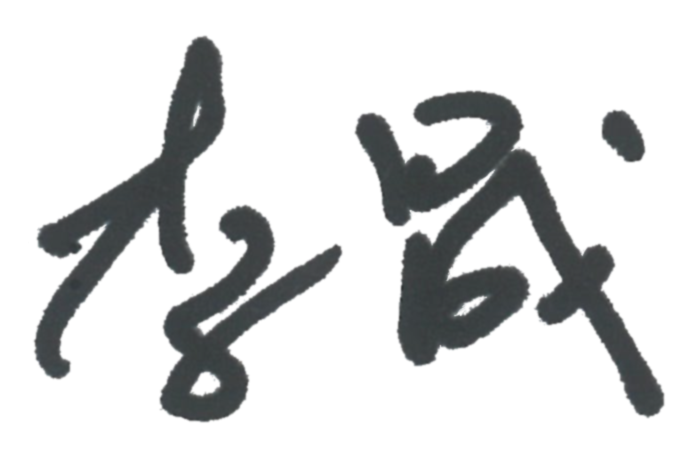
\includegraphics[width=4em]{lisheng.png}}}$\par
~\par
\begin{flushright}\chinesedate\today\end{flushright}

\normalsize

\setlength{\parindent}{1.5em}

\maketitle

\begin{abstract}
We have developed a convenient online software that can simulate hamiltonian mechanics.
Users can see the motion of a system as long as he tells the simulator
the hamiltonian of the system and the initial conditions of it.
The simulator can also analyze the oscillation pattern of a oscillator
by using FFT to derive the frequency domain of the motion.
The simulator is small and fast, and is convenient and easy to operate and customize.
The user interface is simple (a graphics interface for simple basic operations
and a console interface for other operations).
The simulator can also output data of the simulated system to create datasets
for other potential usages.
There are a lot of applications that can be done with it.
\end{abstract}

\keywords{hamiltonian, simulation, mechanics, visualization}

\tableofcontents

\section{Introduction}
\label{sec:intro}

Theoretical mechanics is a subject difficult to study.
One can often find that he cannot find out what the motion of a mechanics system looks like,
so he may probably want to see the graph of the motion.
A software that can output the motion of a system as long as the mechanics system is defined is called a mechanics simulator.

There have been a lot of mechanics simulators available on the Internet,
but most of them have one of the following disadvantages:
\begin{enumerate}
  \item Too massive.
  Some simulators are really powerful, but the cost is its massive volume.
  This makes them unportable.

  \item Not convenient enough.
  Most of the simulators require the user to download the program files into the disk.
  This is inconvenient because you have to reinstall the software when you use another device.

  \item Not customizable enough.
  Some simulators focuses on usual models in real life.
  It may be useful when it comes to rigid body contact problems.
  However, it is usually not shipped with functions to simulate systems like arbitrary central force field or special relativity problems.

  \item Unable to output data.
  Some simulators aims at present how the appearance of the system change,
  but they lack a convenient interface to output the very data of the motion of the system.

  \item Too difficult to operate.
  Some powerful simulators have very complicated user interface,
  which requires the user to study for hours to being able to operate the simulator and check the result.
  This is not friendly to new users.
\end{enumerate}

Because of this, we wanted to create a simulator to solve the problems above.
To make it convenient to use, it should be hosted on a webpage
so that everyone with a browser can have access to it as long as he can access the Internet.

With such a simulator, one can study theoretical mechanics more conveniently.
He can have perceptual congnition about specific mechanics systems.
The simulator can also be used as animated presentation for physics education or lecture.

\section{List of symbols}

Note that if a symbol has domain $A\rightarrow B$,
which means a function from set $A$ to set $B$,
then it can sometimes represent the value of the function
and lies in the domain $B$.
In other words, if it says that $f:A\rightarrow B$ is a function w.r.t. $x$,
then $f$ can be a abbreviation of $f\left(x\right)$.

We always assume that functions we encounter have good enough properties as long as we need to use this property.

The list of symbols is shown in Table \ref{tab:symbols}.
The list of mathematical operations is shown in Table \ref{tab:operations}.

Since all quantities are implemented numerically in the computer program as floating numbers,
the quantities do not necessarily share the same units as in the real world
but use other more convenient units like pixel or tick,
so the units are not mentioned in the lists.

There are some model-specific symbols mentioned in examples in Section \ref{sec:program}.
They are not included the the list of symbols, but their specific meanings are explained in the section.

\begin{table}[h]
  \caption{List of symbols}
  \label{tab:symbols}
  \centering
  \begin{tabular}{cccc}
    Symbol & Domain & Meaning & Value\\
    \hline
    $t$ & $\mathbb R$ & Time\\
    $\Delta t$ & $\mathbb R^+$ & The increment step of the ODE solver & $\SI{5e-4}{}$\\
    $\iota$ & $\left\{2\zeta\middle|\zeta\in\mathbb Z^+\right\}$ & The dimension of the vector in the ODE\\
    $\mathbf x$ & $\mathbb R\rightarrow\mathbb R^\iota$ & The state of a system w.r.t. $t$ & $\left(\mathbf q,\mathbf p\right)$\\
    $\mathbf q$ & $\mathbb R\rightarrow\mathbb R^{\iota/2}$ & Generalized coordinates w.r.t. $t$\\
    $\mathbf p$ & $\mathbb R\rightarrow\mathbb R^{\iota/2}$ & Generalized momentum w.r.t. $t$\\
    $\mathcal H$ & $\mathbb R\times\mathbb R^\iota\rightarrow\mathbb R$ & Hamiltonian w.r.t. $\left(t,\mathbf x\right)$\\
    $\boldsymbol\omega$ & $\mathbb R^{\iota\times\iota}$ & A matrix to make symplectic gradients & $\left[\begin{matrix}
      \mathbf O & \mathbf I_{\iota/2}\\
      -\mathbf I_{\iota/2} & \mathbf O
    \end{matrix}\right]$\\
    $\xi$ & $\mathbb R$ & Abscissa on the canvas, in pixel\\
    $\eta$ & $\mathbb R$ & Ordinate on the canvas, in pixel\\
    $m_t$ & $\mathbb R\rightarrow\mathbb R$ & \makecell{The mapping from actual $t$\\to the $\xi$-coordinate on the canvas}\\
    $m_y$ & $\mathbb R\rightarrow\mathbb R$ & \makecell{The mapping from actual $\mathbf x$ component\\to the $\eta$-coordinate on the canvas}\\
    $w$ & $\mathbb Z^+$ & The width of the graphics screen & $1024$\\
    $h$ & $\mathbb Z^+$ & The height of the graphics screen & $768$\\
    $y$ & $\mathbb R$ & The component of $\mathbf x$ to be plotted\\
    $N$ & $\mathbb Z^+$ & Number of samples to calculate DFT & $\SI{1e5}{}$\\
    $W$ & $\left[0,1\right)\rightarrow\mathbb R$ & The window function & See Equation \ref{eq:hamming}
  \end{tabular}
\end{table}

\begin{table}[h]
  \caption{List of operations}
  \label{tab:operations}
  \centering
  \begin{tabular}{ccc}
    Symbol & Name & Definition\\
    \hline
    $\dot f$ & Complete derivative\tablefootnote{
      \label{fn:complete}Complete derivative means that:
      if $f$ is a function w.r.t. $g$, and $g$ is a function w.r.t. $t$,
      then $\dot f$ denotes $\frac{\mathrm d}{\mathrm dt}f\left(g\left(t\right)\right)$.
    } of $f$ w.r.t. $t$ & $\frac{\mathrm df}{\mathrm dt}$\\
    $\Delta f$ & Complete change\tablefootnote{
      Complete change is similar to complete derivative. See Footnote \ref{fn:complete}. 
    } in $f$ when $t$ becomes $t+\Delta t$ & $f\left(t+\Delta t\right)-f\left(t\right)$\\
    $\sum_j^nr_j$ & Sum of $n$ numbers w.r.t. index $j$\tablefootnote{
      By conventions in computer science, indices start from $0$ instead of $1$.
      The convention will be followed in the article.
    } & $\sum_{j=0}^{n-1}r_j$\\
    $\zeta\mathbin\%\chi$\tablefootnote{
      This notation is from conventions in computer science.
    } & Remainder of $\zeta$ divided by $\chi$ & $\zeta-\chi\left\lfloor\frac\zeta\chi\right\rfloor$
  \end{tabular}
\end{table}

\section{Physics theory}
\label{sec:theory}

\subsection{Predicting dynamics}

A dynamics system's motion can be predicted using some ordinary differential equations (ODE) in form of
\begin{equation}
  \dot{\mathbf x}=\mathbf f\left(t,\mathbf x\right),
  \label{eq:ode}
\end{equation}
where $\mathbf f:\mathbb R\times\mathbb R^\iota\mapsto\mathbb R^\iota$
is a function related to the specific system,
and $\iota$ is some positive integer which should unnecessarily
be the degree of freedom (DOF) of the system (it is actually 2 times DOF in our case).

\subsection{ODE solver}
\label{sec:ode_solver}

\VerbatimFootnotes
This ODE (Equation \ref{eq:ode}) can be solved numerically using the Runge--Kutta method\footnote{
  The algorithm can be expressed more briefly using Ruby programming language:
  \begin{minted}{ruby}
  dx = b.zip(a).each_with_object([]).sum do |(bj, aj), ary|
    bj * ary.push(f.(t+aj.sum*dt, x+aj.zip(ary).sum{_1*_2}*dt)).last
  end * dt
  \end{minted}
}

\begin{equation}
  \Delta\mathbf x\approx\Delta t\sum_j^sb_j\mathbf K_j,
\end{equation}
where $\mathbf K_j$ is defined recursively as \cite[p. 907]{press2007numerical}
\begin{equation}
  \mathbf K_j:=f\left(t+\Delta t\sum_k^ja_{j,k},\mathbf x+\Delta t\sum_k^ja_{j,k}\mathbf K_k\right).
\end{equation}
The smaller $\Delta t$ is, the more precise and the less efficient the solver is.

The order number $s$ and the coefficients $b_j$ and $a_{j,k}$
are specific for different Runge--Kutta methods.
Here the 3/8-rule \cite[p. 138]{hairer2008solvingODE} is adopted.
The coefficients of it is shown in Table \ref{tab:3/8-rule}.

\begin{table}[h]
  \caption{The coefficients of Runge--Kutta method 3/8-rule}
  \label{tab:3/8-rule}
  \centering
  \begin{tabular}{c|cccc|c}
    & \multicolumn{4}{c|}{$a_{j,k}$} & $b_j$\\
    \hline
    \diaghead{\theadfont DiagDia}{$j$}{$k$} & $0$ & $1$ & $2$ & $3$\\
    \hline
    $0$ &        &      &     & & $1/6$\\
    $1$ & $1/3$  &      &     & & $1/3$\\
    $2$ & $-1/3$ & $1$  &     & & $1/3$\\
    $3$ & $1$    & $-1$ & $1$ & & $1/8$
  \end{tabular}
\end{table}

The ODE solver should store $t$ and $\mathbf x$,
and every time it increments, log $\left(t,\mathbf x\right)$ and
let $\mathbf x\leftarrow\mathbf x+\Delta\mathbf x$ and $t\leftarrow t+\Delta t$.

The ODE solver can give the numerical value of $\mathbf x$ at any $t$
as long as the numerical form of $\mathbf f$
and a initial value $\mathbf x\left(0\right)$
is given.

\subsection{Constructing ODE}

Only an ODE solver does not help with simulating a dynamics.
The ODE is required.
According to the theorems in physics,
there are a lot of methods to construct the ODE of a dynamics system.
Here the hamiltonian method is adopted.

The hamiltonian mechanics states that, for some dynamics system,
there exists a function
$\mathcal H:\mathbb R^\iota\times\mathbb R\rightarrow\mathbb R:\left(t,\mathbf x\right)\mapsto\mathcal H\left(t,\mathbf x\right)$
such that the motion of the system satisfy the equation
called \textbf{canonical equation}\footnote{
  The canonical equation is usually denoted as
  \begin{equation*}
    \dot{\mathbf q}=\frac{\partial\mathcal H}{\partial\mathbf p},
    \quad
    \dot{\mathbf p}=-\frac{\partial\mathcal H}{\partial\mathbf q}
  \end{equation*}
  in other books \cite{hand2008mechanics}\cite[p. 65]{arnold1989mathmech}\cite[p. 132]{landau1976mechanics}.
}
\begin{equation}
  \dot{\mathbf x}=\boldsymbol\omega\nabla_{\mathbf x}\mathcal H,
\end{equation}
where $\boldsymbol\omega\nabla_{\mathbf x}$ denotes the \textbf{symplectic gradient} w.r.t. $\mathbf x$.

Under the circumstance of hamiltonian mechanics,
the vector $\mathbf x\in\mathbb R^\iota$ can be separated into two vectors
$\mathbf q\in\mathbb R^{\iota/2}$ and $\mathbf p\in\mathbb R^{\iota/2}$,
which are respectively the \textbf{generalized coordinates} and \textbf{generalized momentum} of the system,
so the components of $\mathbf x$ can be called \mintinline{js}{q0}, \mintinline{js}{q1}, \mintinline{js}{p0}, \mintinline{js}{p1}, etc..

Since the gradient $\nabla_{\mathbf x}\mathcal H$ can be calculated numerically easily,
we can give the numerical form of $\mathbf f$ in Equation \ref{eq:ode} according to
\begin{equation}
  \mathbf f\left(t,\mathbf x\right):=\boldsymbol\omega\nabla_{\mathbf x}\mathcal H
  \label{eq:def_f}
\end{equation}
and can thus solve Equation \ref{eq:ode} numerically according to the method described in Section \ref{sec:ode_solver}.

\subsection{Analyzing the frequency domain of the motion}
\label{sec:theory_fft}

When we study the periodical motion of a dynamics system,
it is usually interesting to study its frequency domain.
Therefore, we want the simulator to be shipped with the ability
to show the Fourier transformation (FT) of the motion
(on an interval of time $\left[0,N\Delta t\right)$).
Because we do this numerically, and $t$ is actually discrete,
so what we calculate is actually the discrete Fourier transformation (DFT).

The FFT library mentioned in Section \ref{sec:fft} provides the method
to calculate the DFT.
Although we can just pick a time interval long enough and calculate its DFT,
the operation can result in some loss in the frequency domain \cite{harris1978ft}.
We should apply a window function to the motion on the interval before calculating DFT.

There are various window functions candidates,
each of which have its unique application scenes.
Here the Hamming window function \cite{harris1978ft}
\begin{equation}
  W\left(\zeta\right):=\frac{25}{46}-\frac{21}{46}\cos\left(2\pi\zeta\right)
  \label{eq:hamming}
\end{equation}
is adopted because it fits with most cases.

\begin{figure}[h]
  \centering
  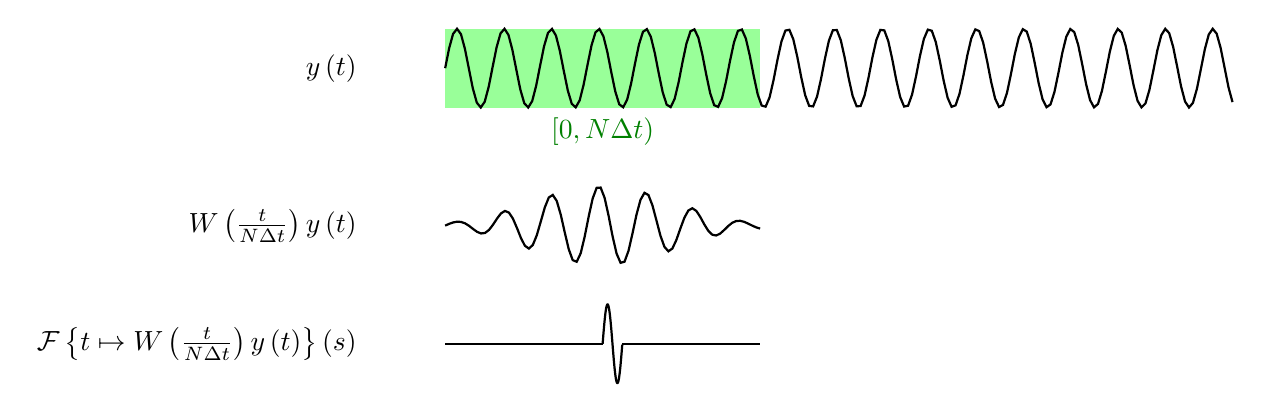
\begin{tikzpicture}
    \node[left] at (-1,-1) {$y\left(t\right)$};
    \fill[green!40!white] (0,-0.5) rectangle +(4,-1);
    \node[below,text=green!50!black] at (2,-1.5) {$\left[0,N\Delta t\right)$};
    \draw[thick,domain=0:10,samples=200,variable=\x] plot ({\x},{0.5*sin(600*\x)-1});
    \node[left] at (-1,-3) {$W\left(\frac t{N\Delta t}\right)y\left(t\right)$};
    \draw[thick,domain=0:4,samples=80,variable=\x] plot ({\x},{(25/46-21/46*cos(360*\x/4))*0.5*sin(600*\x)-3});
    \node[left] at (-1,-4.5) {$\mathcal F\left\{t\mapsto W\left(\frac t{N\Delta t}\right)y\left(t\right)\right\}\left(s\right)$};
    \draw[thick,domain=2:2.25,samples=200,variable=\x] plot ({\x},{0.5*sin(1440*\x)-4.5});
    \draw[thick] (0,-4.5) -- (2,-4.5);
    \draw[thick] (2.25,-4.5) -- (4,-4.5);
  \end{tikzpicture}
  \caption{The process of deriving the frequency domain}
  \label{fig:fft}
\end{figure}

\section{Libraries used by the simulator}

Our simulator depends on some third-party libraries.

The graphics library is used to show graphs on the screen.

The FFT library is used to calculate the DFT of the motion of the system.

The ODE constructor and ODE solver is written by us,
independent to third-party libraries.
The theories about them are explained in Section \ref{sec:theory}.

\subsection{Graphics library}

We use rpg\_core.js to draw and show graphs.
It is a web game engine based on \href{https://www.pixijs.com}{PixiJS}.
Although rpg\_core.js is shipped with \href{https://tkool.jp/mv}{RPG Maker MV},
which is not a free software,
it is open-source \href{https://github.com/rpgtkoolmv/corescript}{on GitHub}.

In rpg\_core.js, a \mintinline{js}{Bitmap} object is used to store the info of a picture,
and a \mintinline{js}{Sprite} object is used to present the picture depicted by a \mintinline{js}{Bitmap}.
The coordinates info etc. are also in the \mintinline{js}{Sprite} \cite{rmmvhelp}.
Figure \ref{fig:show_picture} shows how rpg\_core.js shows a picture.

\begin{figure}[h]
  \centering
  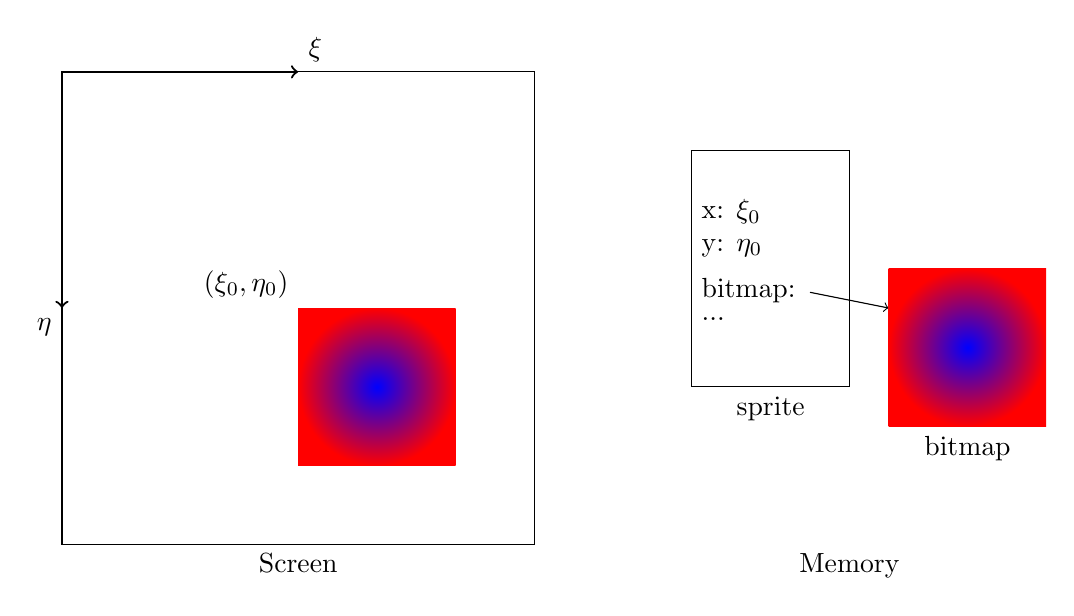
\begin{tikzpicture}
    \draw (0,0) rectangle +(6,-6);
    \node[below] at (3,-6) {Screen};
    \draw[thick,->] (0,0) -- +(3,0) node[anchor=south west] {$\xi$};
    \draw[thick,->] (0,0) -- +(0,-3) node[anchor=north east] {$\eta$};
    \shade[inner color=blue,outer color=red] (3,-3) rectangle +(2,-2);
    \node[above left] at (3,-3) {$\left(\xi_0,\eta_0\right)$};

    \node[below] at (10,-6) {Memory};
    \draw (8,-1) rectangle +(2,-3);
    \node[below] at (9,-4) {sprite};
    \node[below right] at (8,-1.5) {x: $\xi_0$};
    \node[below right] at (8,-2) {y: $\eta_0$};
    \node[below right] at (8,-2.5) {bitmap:};
    \node[below right] at (8,-3) {...};
    \draw[->] (9.5,-2.8) -- (10.5,-3);
    \shade[inner color=blue,outer color=red] (10.5,-2.5) rectangle +(2,-2);
    \node[below] at (11.5,-4.5) {bitmap};
  \end{tikzpicture}
  \caption{How rpg\_core.js shows a picture}
  \label{fig:show_picture}
\end{figure}

The \mintinline{js}{x} and \mintinline{js}{y} property of a \mintinline{js}{Sprite} can be adjusted to move a picture.

rpg\_core.js also provides methods to fill a rectangular region on a \mintinline{js}{Bitmap}
with a certain color.
This enables us to set the color of pixels on a \mintinline{js}{Bitmap} and can thus draw graphs.

\subsection{FFT library}
\label{sec:fft}

A FFT library implements the fast Fourier transformation (FFT) algorithm.
The FFT library we use is \href{http://www.fftw.org}{FFTW}, which is written in C.
Since we need to use it on the webpage,
we used \href{https://emscripten.org}{emscripten} to import it.

\section{Plotting the graph}

According to the theories described in Section \ref{sec:theory},
a program can be designed to give
the generalized coordinates $\mathbf q$ and generalized momentum $\mathbf p$ at any $t$
according to the input hamiltonian $\mathcal H$
and initial values $\mathbf q\left(0\right)$ and $\mathbf p\left(0\right)$.

However, a person can hardly figure out the patterns in the motion
by just looking at a bunch of $\left(t,\mathbf x\right)$ pairs.
To make it easier to find out the patterns,
the simulator should be capable of plotting a graph
according to the $\left(t,\mathbf x\right)$ pairs.

To be more specific, for each component $y$ of $\mathbf x$,
on the $\xi$-$\eta$ plane (the canvas),
the point $\left(m_t\left(t\right),m_y\left(y\right)\right)$ should be plotted.
The introduction of $m_t$ and $m_y$ is because the coordinates on the canvas
are in pixel, which is a small unit.
Another purpose of $m_t$ and $m_y$ is to make it possible to use nonlinear
scales like logarithmic scale.

\subsection{Scrolling the graph}

Since people often want to simulate a system for a long time,
which makes the graph very wide,
so the canvas should be much wider than the screen.
Then we must make the canvas scroll as the simulator simulates the system.

Although nowadays computers can draw pictures on the screen very fast
and can redraw it every $1/60$ seconds,
the read-write operations to the \mintinline{js}{Bitmap} is time-consuming.
Therefore, here we implement a scroll algorithm similar to Carmack scroll algorithm.
Using this method, the computer only need to change one pixel
on the \mintinline{js}{Bitmap} instead of tens of thousands of them
every time when the ODE solver increments.

The algorithm requires 2 sprites, respectively called sprite 1 and sprite 2,
both of which shows a bitmap of width $w$ and height $h$
(so there are 2 bitmaps altogether),
where $w$ and $h$ are also the width and height of the graphics screen.

\begin{figure}[h]
  \centering
  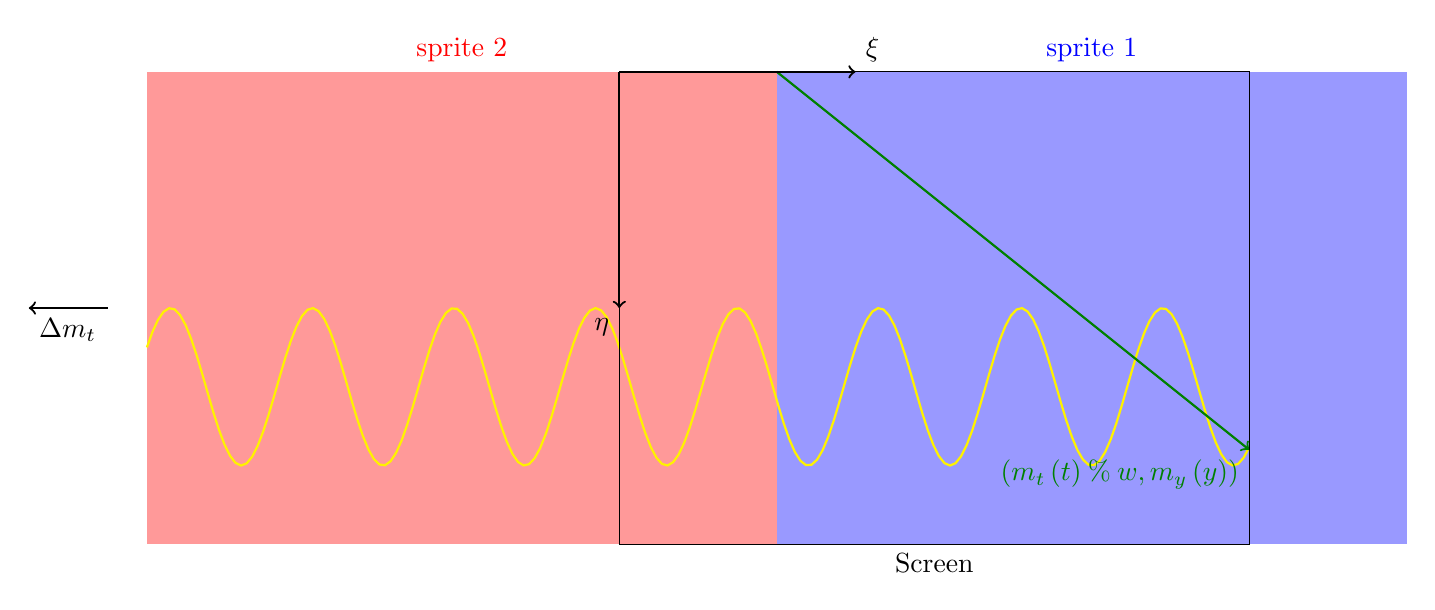
\begin{tikzpicture}
    \fill[blue!40!white] (2,0) rectangle +(8,-6);
    \node[above,text=blue] at (6,0) {sprite 1};
    \fill[red!40!white] (-6,0) rectangle +(8,-6);
    \node[above,text=red] at (-2,0) {sprite 2};
    \draw[thick,domain=-6:8,samples=200,variable=\x,yellow] plot ({\x},{sin(200*\x+150)-4});
    \draw[thick,->,green!50!black,text=green!50!black] (2,0) -- (8,-4.8) node[anchor=north east] {$\left(m_t\left(t\right)\mathbin\%w,m_y\left(y\right)\right)$};
    \draw (0,0) rectangle +(8,-6);
    \node[below] at (4,-6) {Screen};
    \draw[thick,->] (0,0) -- +(3,0) node[anchor=south west] {$\xi$};
    \draw[thick,->] (0,0) -- +(0,-3) node[anchor=north east] {$\eta$};
    \draw[thick,->] (-6.5,-3) -- +(-1,0) node[anchor=north west] {$\Delta m_t$};
  \end{tikzpicture}
  \caption{How the sprites move and the bitmaps are plotted as the ODE solver increments}
  \label{fig:scrolling}
\end{figure}

When the ODE solver increments,
sprite 1 and sprite 2 move left by $\Delta m_t$.
Now, the coordinates of sprite 1 are $\left(w-\left(m_t\left(t\right)\mathbin\%w\right),0\right)$,
and the coordinates of sprite 2 are $\left(-\left(m_t\left(t\right)\mathbin\%w\right),0\right)$.
Fill the pixel at $\left(m_t\left(t\right)\mathbin\%w,m_y\left(y\right)\right)$
on the bitmap of sprite 1.
This process is shown in Figure \ref{fig:scrolling}.

When the two sprites move left enough,
sprite 1 touches the left side of the screen.
At this moment, sprite 2 suddenly moves to the right to sprite 1,
clears its bitmap,
and exchange its name with sprite 1.
This process is shown in Figure \ref{fig:switching}.

\begin{figure}[h]
  \centering
  \begin{subfigure}[b]{\linewidth}
    \centering
    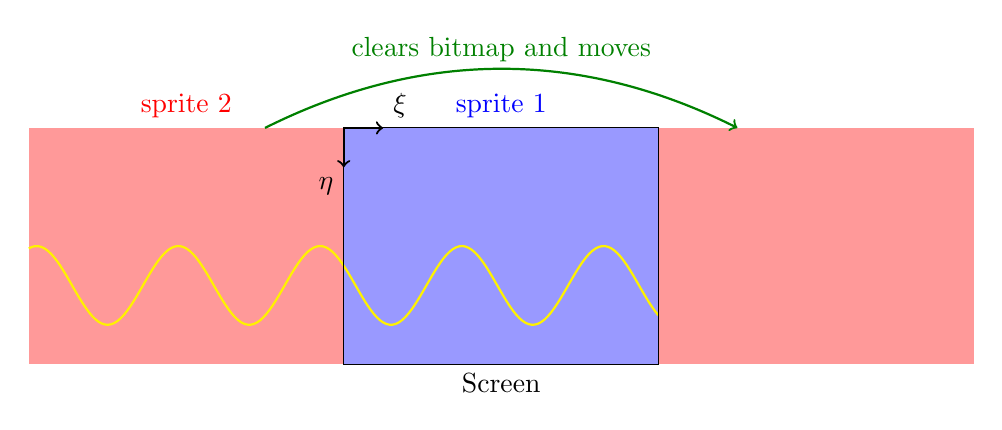
\begin{tikzpicture}
      \fill[blue!40!white] (0,0) rectangle +(4,-3);
      \node[above,text=blue] at (2,0) {sprite 1};
      \fill[red!40!white] (-4,0) rectangle +(4,-3);
      \node[above,text=red] at (-2,0) {sprite 2};
      \fill[red!40!white] (4,0) rectangle +(4,-3);
      \draw[thick,->,green!50!black] (-1,0) .. controls (1,1) and (3,1) .. (5,0);
      \node[text=green!50!black] at (2,1) {clears bitmap and moves};
      \draw[thick,domain=-4:4,samples=200,variable=\x,yellow] plot ({\x},{0.5*sin(200*\x+150)-2});
      \draw (0,0) rectangle +(4,-3);
      \node[below] at (2,-3) {Screen};
      \draw[thick,->] (0,0) -- +(0.5,0) node[anchor=south west] {$\xi$};
      \draw[thick,->] (0,0) -- +(0,-0.5) node[anchor=north east] {$\eta$};
    \end{tikzpicture}
    \caption{Sprite 2 suddenly clears its bitmap and moves}
  \end{subfigure}
  \begin{subfigure}[b]{\linewidth}
    \centering
    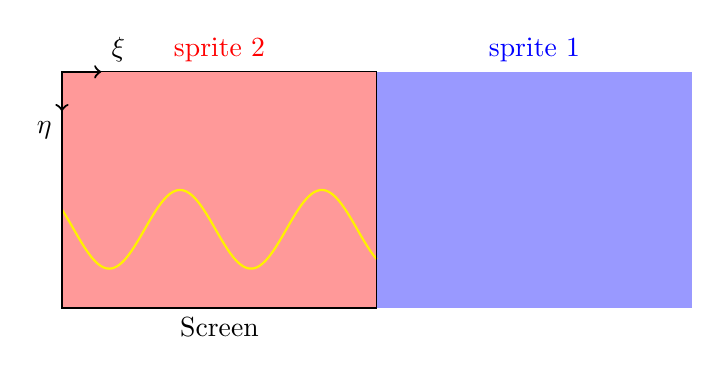
\begin{tikzpicture}
      \fill[red!40!white] (0,0) rectangle +(4,-3);
      \node[above,text=red] at (2,0) {sprite 2};
      \fill[blue!40!white] (4,0) rectangle +(4,-3);
      \node[above,text=blue] at (6,0) {sprite 1};
      \draw[thick,domain=0:4,samples=100,variable=\x,yellow] plot ({\x},{0.5*sin(200*\x+150)-2});
      \draw (0,0) rectangle +(4,-3);
      \node[below] at (2,-3) {Screen};
      \draw[thick,->] (0,0) -- +(0.5,0) node[anchor=south west] {$\xi$};
      \draw[thick,->] (0,0) -- +(0,-0.5) node[anchor=north east] {$\eta$};
    \end{tikzpicture}
    \caption{Sprite 1 and sprite 2 swap their names}
  \end{subfigure}
  \caption{How the sprites suddenly move and swap}
  \label{fig:switching}
\end{figure}

\begin{figure}
  \centering
  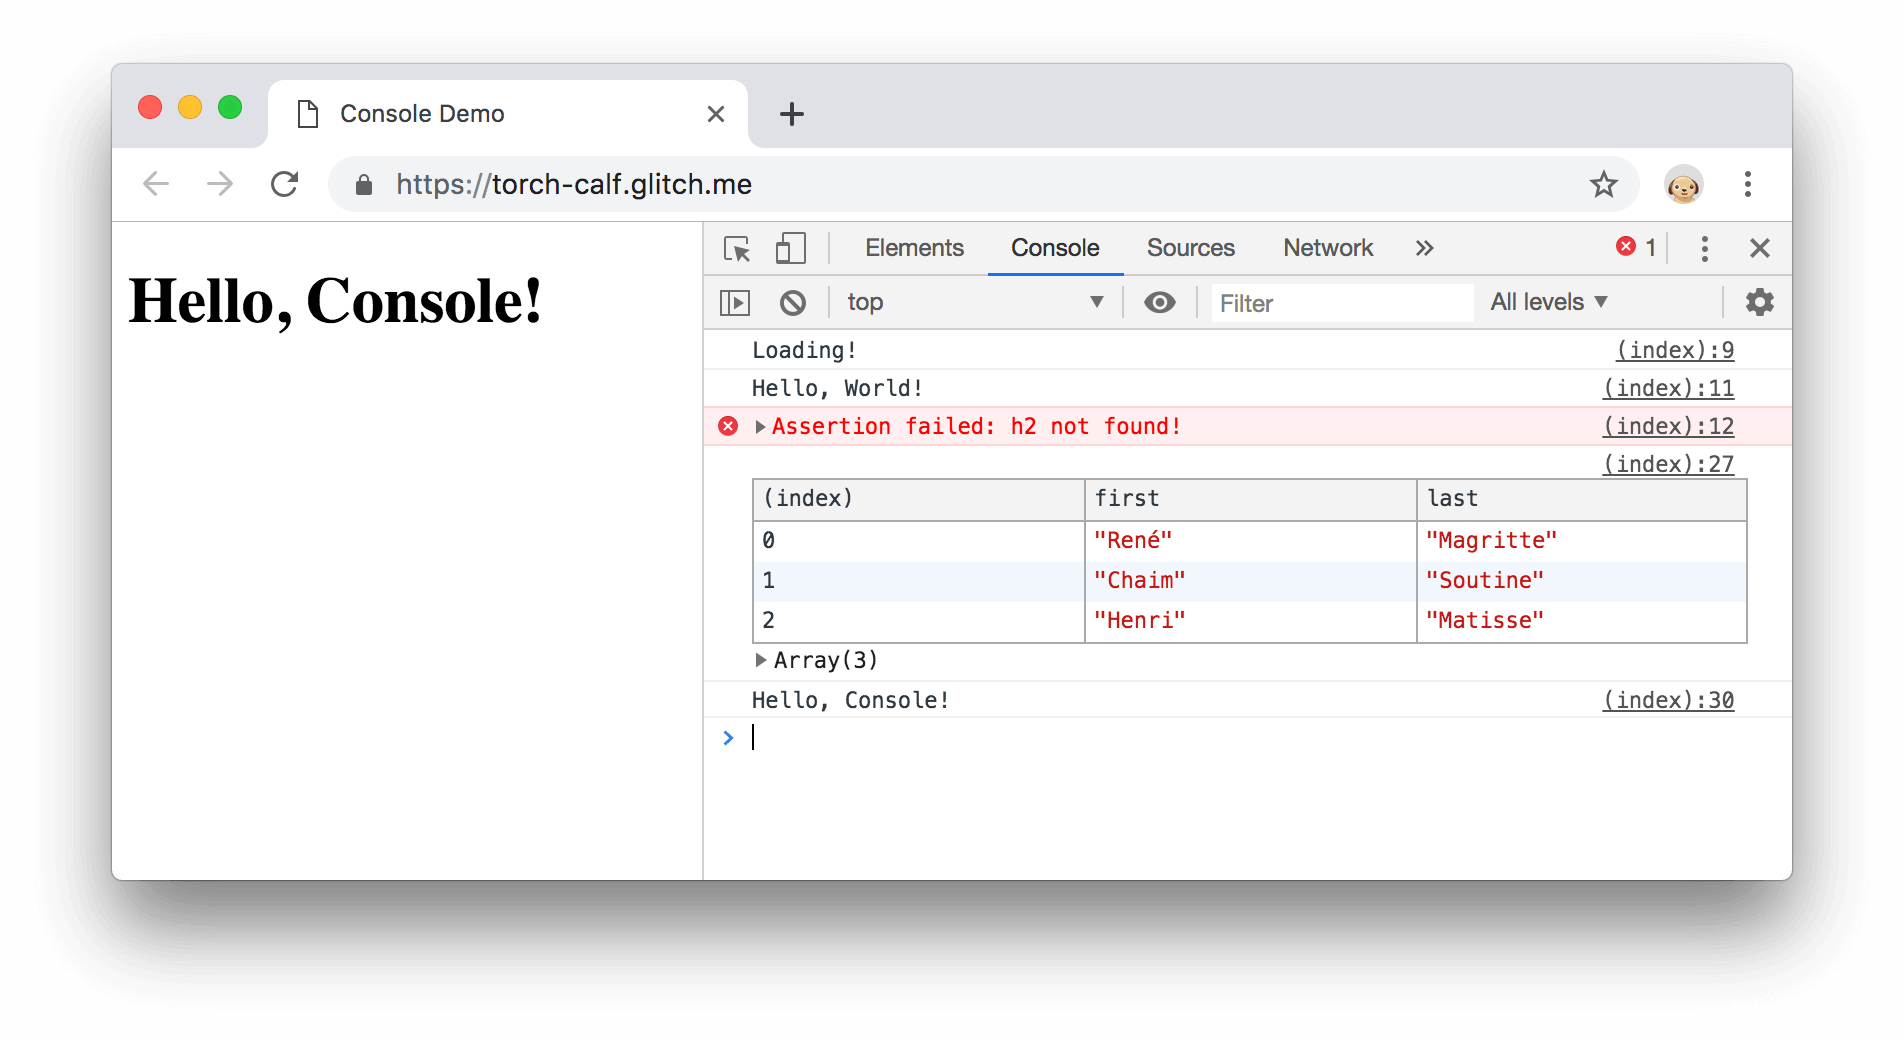
\includegraphics[width=0.9\linewidth]{console_panel.png}
  \caption{The console panel of Chrome browser \cite{chromeconsole}}
  \label{fig:console}
\end{figure}

\subsection{Presenting the frequency domain of the motion}

In Section \ref{sec:theory_fft},
it is said that we need to be able to analyze the frequency domain of the motion.
Since the frequency domain is often discrete and sparse,
and the high-frequency region is often almost zero,
it is better to spread out the low-frequency region across the width of the screen
and connect adjacent points with lines.

Because rpg\_core.js does not ship with a method drawing a straight line on the bitmap,
we need to implement an algorithm to draw straight lines.
Here Bresenham's line algorithm \cite{gaol2013bresenham} is adopted.

\section{Guides for operating}
\label{sec:program}

When you open the \href{https://UlyssesZh.github.io/rpg/mechsimul2}{webpage},
it will start simulating the default model,
which is a 1-dimensional vibration with parametric vibration \cite[p. 82]{landau1976mechanics} and alternating external force \cite[p. 61]{landau1976mechanics}
\begin{equation}
  \mathcal H\left(t,q,p\right)=\frac{p^2}2+\omega^2\left(1+u\cos\left(\gamma t\right)\right)\frac{q^2}2-fq\cos\left(\kappa t+\beta\right),
\end{equation}
where
\begin{equation*}
  \left(u,\gamma,\beta,\kappa,\omega,f\right)=\left(0.3,21.7,0.2,8,10,20\right),
\end{equation*}
and the initial conditions are
\begin{equation*}
  \left(q,p\right)=\left(2,0\right).
\end{equation*}

\begin{figure}[h]
  \centering
  \begin{subfigure}[b]{0.45\linewidth}
    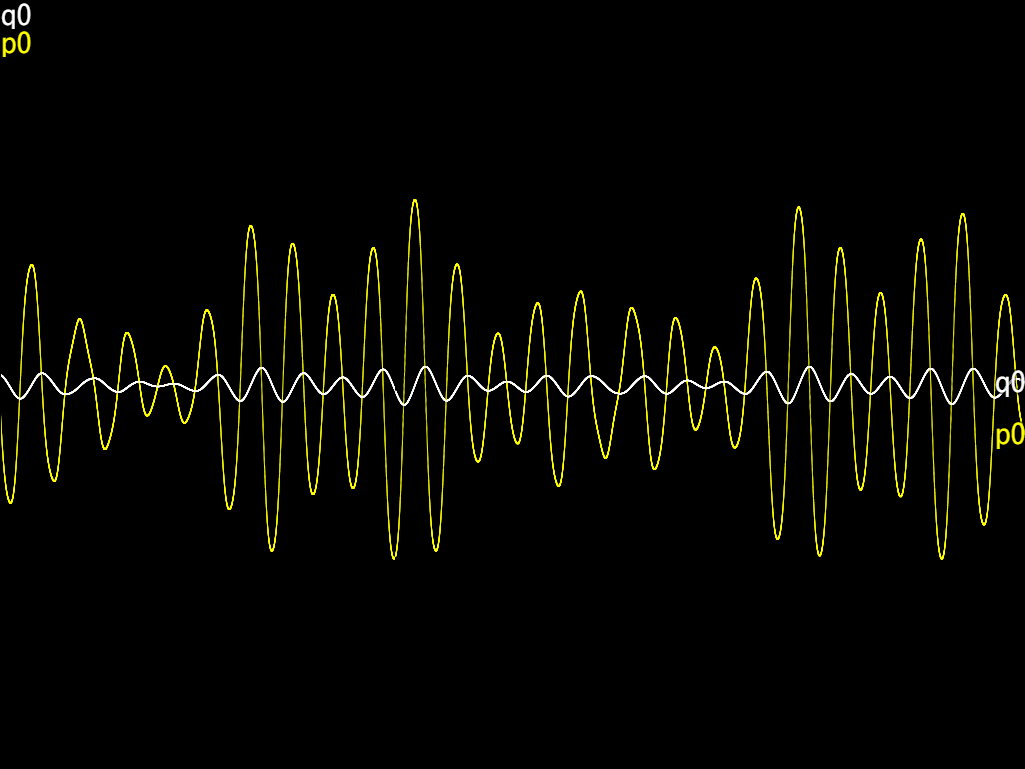
\includegraphics[width=\linewidth]{default_motion.png}
    \caption{The simulated motion of the default model}
  \end{subfigure}
  \begin{subfigure}[b]{0.45\linewidth}
    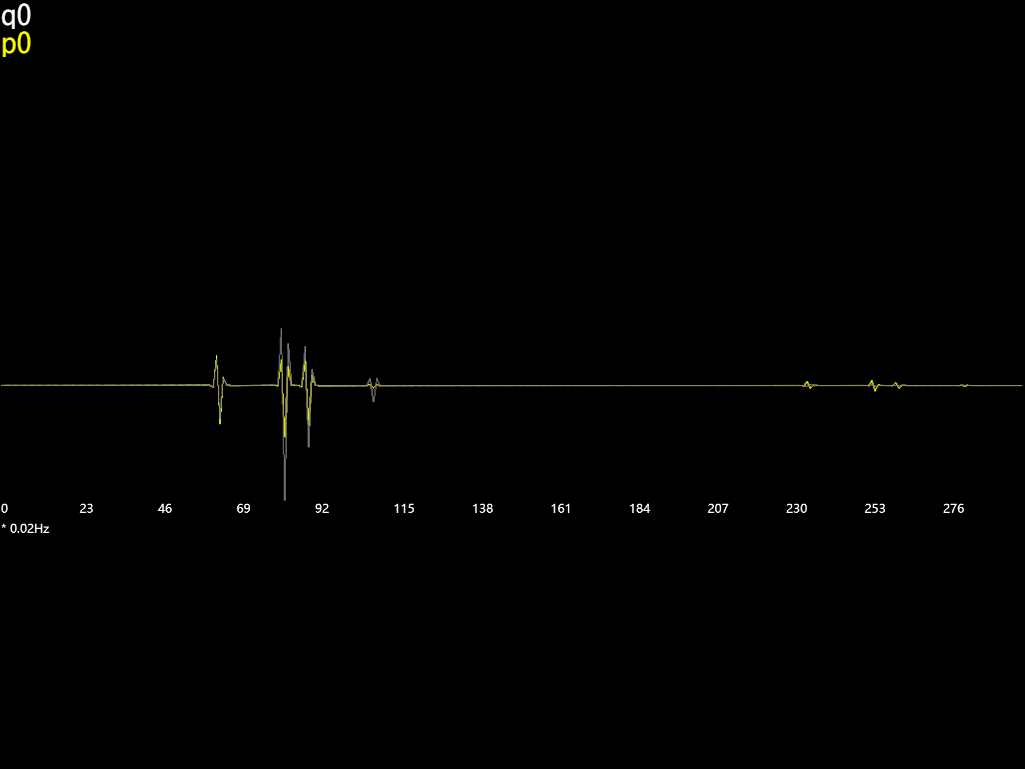
\includegraphics[width=\linewidth]{default_p0_frequencies.png}
    \caption{The frequency domain of $p$ of the default model}
  \end{subfigure}
  \caption{The screenshots of the simulator simulating the default model}
  \label{fig:default}
\end{figure}

The frequency domain calculator feature is enabled.
After some time, when there have accumulated enough samples,
the simulator will create buttons at the up-left corner of the screen
clicking which will make it show the time domain to be FFTed
and the calculated frequency domain.

In the interface of frequency domain,
the line colored the same as the button represents the real part of the FFT result,
and the line colored gray represents the imaginary part of the FFT result.

Hit \LKeySpace ~to pause or resume the simulation.

Figure \ref{fig:default} shows the graphics interface of the simulator.
From the result of the simulation,
it seems that we can indeed learn something about the pattern of the motion.
The frequency domain is very clear.

As described in Section \ref{sec:intro}, the simulator is highly customizable.
You can customize the simulation by coding in the console\footnote{
  For most browsers, hit \LKeyF{12} to have access to the console.
  The interface of the console panel usually looks like Figure \ref{fig:console}.
}.

\subsection{Downloading the motion data}

The simulator will not record the history of the ODE solver by default.
To ask the simulator to record the history, run the following codes.

\begin{minted}{js}
  rungeKutta.recordHistory = true;
  restart();
\end{minted}

Wait the ODE solver for some time for it to accumulate enough data,
and then run the following codes to download the simulated data.

\begin{minted}{js}
  rungeKutta.downloadHistory(0, 30);
\end{minted}

Replace \mintinline{js}{0} and \mintinline{js}{30} with the ends of interval of time
during which your desired data was simulated out.
Omitting the 2 parameters will make it download all data accumulated so far.

\subsection{Changing the parameters of the default model}

For instance, now we want to study the pattern of parametric resonance.
For a parametric vibration model, when $\gamma\approx2\omega$,
the condition for it to reach parametric resonance is\footnote{
  Precision to $\mathrm O\left(u\right)$.
} \cite[p. 82]{landau1976mechanics}
\begin{equation}
  \left|\gamma-2\omega\right|<\frac12\omega u.
\end{equation}

We want to study how the motion looks like when it reaches parametric resonance.
We can let $f:=0$ to cancel the external force
and let $\gamma:=21.3$ to make the system meet the condition of parametric resonance.
Then, run \mintinline{js}{restart()}.

\begin{minted}{js}
  f = 0;
  gamma = 21.3;
  restart();
\end{minted}

\subsection{Changing the initial conditions}

The initial conditions $\mathbf x\left(0\right)$ can be set to a customized one
by running the following codes.

\begin{minted}{js}
  rungeKutta.initial = [2, 0];
  restart();
\end{minted}

Change \mintinline{js}{[2, 0]} into any initial conditions you like.

\subsection{Changing the scale}

It can be found that the amplitude indeed grows in an exponential pattern as predicted by theorems.
Since exponential growth is very fast, the graph soon exceeds the screen.
We can use logarithmic scale to prevent this.
This can be done by changing $m_y$ using the following codes.

\begin{minted}{js}
  canvas.mappingY = y => 20 * log1p(abs(y)) * sign(y) + Graphics.height/2;
  restart();
\end{minted}

Now $m_y\left(y\right):=20\ln\left(1+\left|y\right|\right)\operatorname{sgn}y+h/2$.
Note that in the codes, \mintinline{js}{Graphics.width} stands for $w$
and \mintinline{js}{Graphics.height} stands for $h$.

The result of the simulation of the parametric resonance can be seen in Figure \ref{fig:parametric}.
It can be seen that the amplitude is indeed growing exponentially.

\begin{figure}[h]
  \centering
  \begin{subfigure}[b]{0.45\linewidth}
    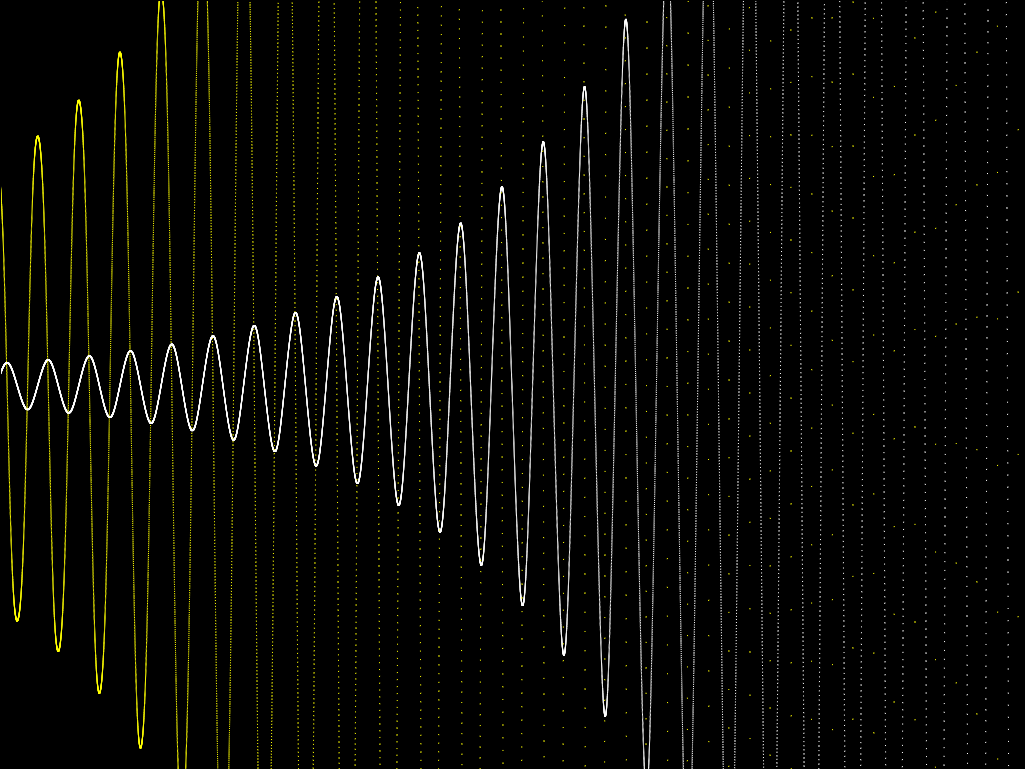
\includegraphics[width=\linewidth]{parametric_resonance.png}
    \caption{The parametric resonance phenomenon is simulated}
  \end{subfigure}
  \begin{subfigure}[b]{0.45\linewidth}
    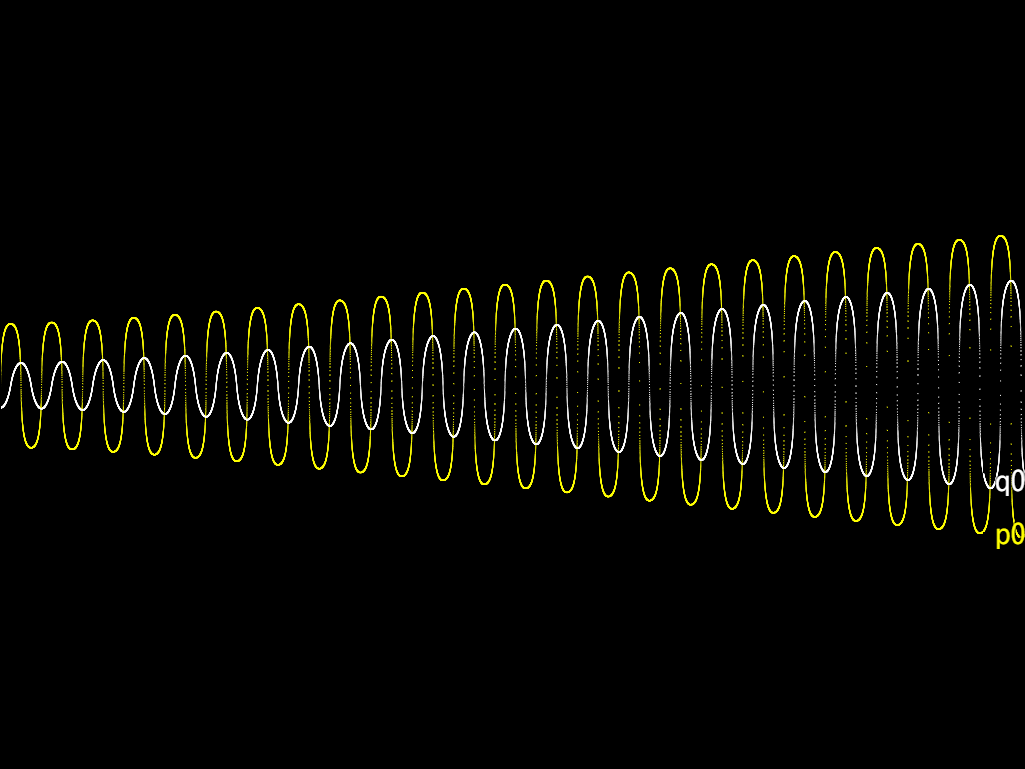
\includegraphics[width=\linewidth]{parametric_resonance_logarithmic.png}
    \caption{Using logarithmic scale to prevent the amplitude growing too fast}
  \end{subfigure}
  \caption{The simulator simulating the parametric resonance}
  \label{fig:parametric}
\end{figure}

\subsection{Disabling analysis of frequency domain}

You can also disable the frequency domain analysis using the following codes.
After running the codes, there will not be buttons appearing at the up-left corner
to indicate the availability of the frequency domain.

\begin{minted}{js}
  canvas.detectPeriod = false;
  restart();
\end{minted}

\subsection{Advanced: drawing the phase path}

A phase path is the graph representing the motion of the phase point $\mathbf x$ \cite[p. 146]{landau1976mechanics}\cite[p. 68]{arnold1989mathmech}.

The simulator has an API to allow the user to run custom codes as the ODE solver increments.
To draw the phase path, first you need to create a \mintinline{js}{Sprite} and a \mintinline{js}{Bitmap}
by following the codes below.

\begin{minted}{js}
  var phaseSprite = new Sprite();
  phaseSprite.bitmap = new Bitmap(Graphics.width, Graphics.height);
  scene.addChild(phaseSprite);
\end{minted}

Then, change \mintinline{js}{canvas.onTrace} to run custom codes when a new point is added,
and \mintinline{js}{restart()}.

\begin{minted}{js}
  canvas.onTrace = (t, qp) => {
    phaseSprite.bitmap.setPixel(...qp.map(canvas.mappingY), 'white');
    return true;
  };
  restart();
\end{minted}

If you want, you can hide the original canvas by running \mintinline{js}{canvas.visible = false;},
and you can clear the phase path at any time by running \mintinline{js}{phaseSprite.bitmap.clear();}.

\begin{figure}
  \centering
  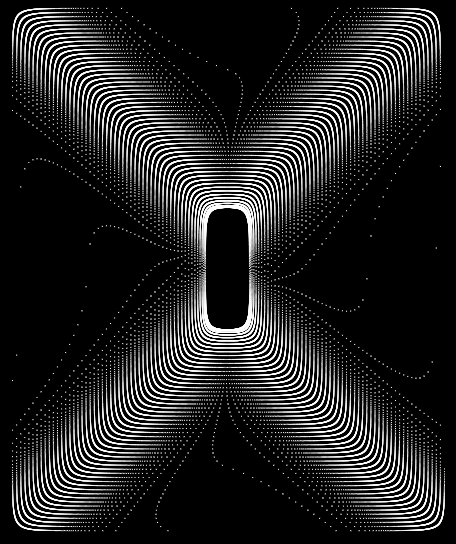
\includegraphics[width=0.3\linewidth]{parametric_resonance_logarithmic_phase.png}
  \caption{The phase path of the parametric resonance in logarithmic scale}
  \label{fig:parametric_phase}
\end{figure}

Figure \ref{fig:parametric_phase} shows the result of the codes above.

The line should be continuous at the edge of each period of the phase path,
but the phase point moves so fast that the simulator cannot trace it continuously.
The discrete points seem to form curves across the phase path,
as can be seen in Figure \ref{fig:parametric_phase}.
What are the equations for them?
It seems that the simulator can inspire us to ask such questions
and encourage us to study something like this about physics.

\subsection{Change the hamiltonian into a nonlinear oscillator}

\begin{figure}
  \centering
  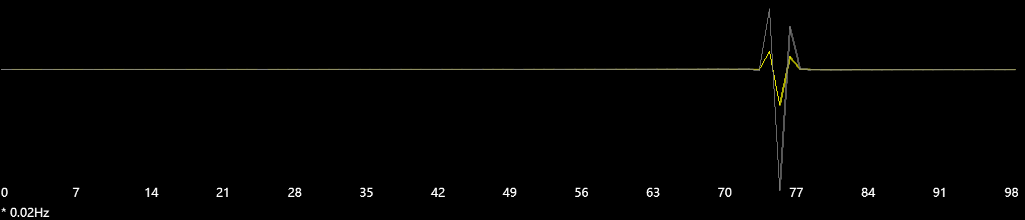
\includegraphics[width=0.9\linewidth]{nonlinear_frequency.png}
  \caption{The frequency spectrum of a nonlinear oscillator (higher frequencies are not shown)}
  \label{fig:nonlinear}
\end{figure}

The user can assign a function value to the variable \mintinline{js}{rungeKutta.func}
to change the $\mathbf f$ in Equation \ref{eq:ode}.
To create the $\mathbf f$ according to the hamiltonian using Equation \ref{eq:def_f},
using the function \mintinline{js}{canonicalEquation},
with the first argument be the DOF, and the second argument be the hamiltonian function.

One example is to change the hamiltonian of the default model into that of a nonlinear oscillator
\begin{equation*}
  \mathcal H\left(t,q,p\right):=\frac{p^2}2+\frac{\omega_0^2q^2}2+\alpha q^3+\beta q^4
\end{equation*}
by running the following codes.
Before applying the codes, if you have runned some codes above,
refresh the webpage\footnote{
  For most browsers, the shortcut of refreshing is to hit \LKeyF{5}.
} to have a clean environment to prevent the modifications above affecting.

\begin{minted}{js}
  rungeKutta.func = canonicalEquation(1, (t, qp) => {
    let [q, p] = qp;
    return p**2/2 + omega0**2*q**2/2 + alpha*q**3 + beta*q**4;
  });
\end{minted}

The parameters $\left(\omega_0,\alpha,\beta\right)$ should be defined.
Assume that we take
\begin{equation*}
  \left(\omega_0,\alpha,\beta\right):=\left(10,-2,-3\right),
\end{equation*}
then we can run the following codes.

\begin{minted}{js}
  var omega0 = 10;
  var alpha = -2;
  var beta = -3;
\end{minted}

If we take the initial conditions as $\left(q,p\right)=\left(1,0\right)$ using the following codes,
the amplitude is now taken as $b=1$.

\begin{minted}{js}
  rungeKutta.initial = [1, 0];
\end{minted}

We can use the simulator to verify the formula for calculating the frequency of the nonlinear oscillator \cite[p. 87]{landau1976mechanics}\footnote{
  Precision to $\mathrm O\left(b^2\right)$.
}
\begin{equation*}
  \omega=\omega_0+\left(\frac{3\beta}{2\omega_0}-\frac{15\alpha^2}{4\omega_0^3}\right)b^2=9.535.
\end{equation*}

The frequency spectrum is shown in Figure \ref{fig:nonlinear}.
As can be seen, the frequency is roughly the theoretically predicted value $\frac\omega{2\pi}=1.518$,
different from the linear one $\frac{\omega_0}{2\pi}=1.592$.

\section{Examples}
\label{sec:examples}

The default model and the typical customizations to it presented in Section \ref{sec:program}
are good examples of the application of the simulator.

Here are some other examples.
The codes of the examples can also be seen on the
\href{https://ulysseszh.github.io/rpg/mechsimul2/examples.html}{webpage}.

\subsection{Kepler's 2-body problem}

2-body problems are systems with $4$ DOF.
The hamiltonian of the model to be simulated is
\begin{equation*}
  \mathcal H\left(t,q_0,q_1,q_2,q_3,p_0,p_1,p_2,p_3\right):=
  p_0^2+p_1^2+p_2^3+p_3^2-\frac{500}{\sqrt{\left(q_0-q_2\right)^2+\left(q_1-q_3\right)^2}}.
\end{equation*}

\begin{figure}[h]
  \centering
  \begin{subfigure}[b]{0.6\linewidth}
    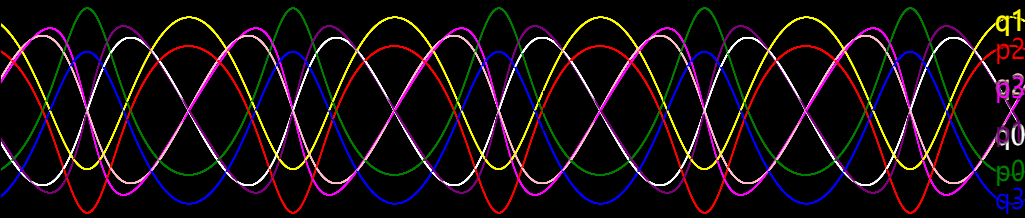
\includegraphics[width=\linewidth]{kepler_2_body_graph.png}
    \caption{The graph of $\mathbf x$, 8 curves in total}
  \end{subfigure}
  \begin{subfigure}[b]{0.15\linewidth}
    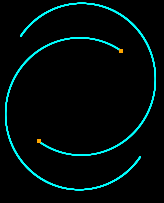
\includegraphics[width=\linewidth]{kepler_2_body_trace.png}
    \caption{Visualization}
  \end{subfigure}
  \begin{subfigure}[b]{0.2\linewidth}
    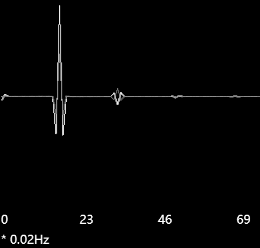
\includegraphics[width=\linewidth]{kepler_2_body_q0_frequencies.png}
    \caption{Frequencies of $q_0$}
  \end{subfigure}
  \caption{The simulator simulating Kepler's 2-body problem}
  \label{fig:kepler}
\end{figure}

Run the following codes and you will get 2 stars move around each other.

\begin{minted}{js}
  // There are 8 curves to be drawn on the canvas
  canvas.n = 8;
  // Setting the hamiltonian of the system
  rungeKutta.func = canonicalEquation(4, (t, qp) => {
    let [x1, y1, x2, y2, px1, py1, px2, py2] = qp;
    return px1**2 + py1**2 + px2**2 + py2**2 - 500 / hypot(x1-x2, y1-y2);
  });
  // Setting the initial conditions of the system
  rungeKutta.initial = [-3, -3, 3, 3, 2, -3, -2, 3];
  // Setting the scale of the graph
  canvas.mappingY = y => 20 * y + Graphics.height/2;
  // Setting the colors for graphing; there are 8 curves and thus 8 colors
  canvas.colors = ["white", "yellow", "pink", "blue",
                   "green", "purple", "red", "magenta"];

  // Following codes creates the sprites and bitmaps for visualization
  // (Using API provided by rpg_core.js, see [1] for help)
  var traceSprite = new Sprite();
  var star1 = new Sprite();
  var star2 = new Sprite();
  scene.addChild(traceSprite);
  scene.addChild(star1);
  scene.addChild(star2);
  traceSprite.bitmap = new Bitmap(Graphics.width, Graphics.height);
  star1.bitmap = star2.bitmap = new Bitmap(4, 4);
  star1.bitmap.fillAll('orange');
  star1.anchor.x = star1.anchor.y = 0.5;
  star2.anchor.x = star2.anchor.y = 0.5;

  // Updating the state of the sprites when a new sample comes out
  canvas.onTrace = (t, qp) => {
    // Setting the position of sprites of stars
    [star1.x, star1.y, star2.x, star2.y] =
        qp.slice(0, 4).map(canvas.mappingY);
    // Plotting the trajectory
    traceSprite.bitmap.setPixel(star1.x, star1.y, 'cyan');
    traceSprite.bitmap.setPixel(star2.x, star2.y, 'cyan');
    return true;
  };

  // Restarting to apply the changes
  restart();
\end{minted}

The simulated result is shown in Figure \ref{fig:kepler}.

If the user is curious, the hamiltonian or the initial conditions can be modified a little to create interesting graphs.

The line \mintinline{js}{rungeKutta.initial = [-3, -3, 3, 3, 5, -2, -5, 2];}
can be modified to apply different initial conditions.
For different initial conditions, the trajectory can appear as a different shape.
If we change \mintinline{js}{2, -3, -2, 3} into \mintinline{js}{5, -2, -5, 2},
the trajectory is hyperbola as shown in Figure \ref{fig:distortion_kepler}.

The line \mintinline{js}{return px1**2 + py1**2 + px2**2 + py2**2 - 500 / hypot(x1-x2, y1-y2);}
can be modified to apply a different hamiltonian to the system.
If you change \mintinline{js}{x1-x2} into \mintinline{js}{1.5*x1-x2},
what you get is a chaotic motion as shown in Figure \ref{fig:distortion_kepler}.

\begin{figure}[h]
  \centering
  \begin{subfigure}[b]{0.4\linewidth}
    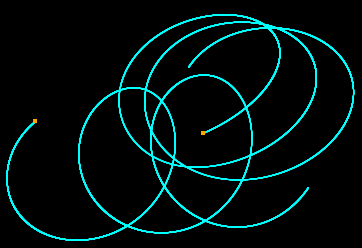
\includegraphics[width=\linewidth]{distortion_kepler.png}
    \caption{The code \mintinline{js}{x1-x2} is changed into \mintinline{js}{1.5*x1-x2}}
  \end{subfigure}
  \begin{subfigure}[b]{0.4\linewidth}
    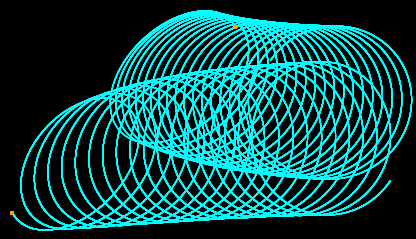
\includegraphics[width=\linewidth]{distortion2_kepler.png}
    \caption{The code \mintinline{js}{x1-x2} is changed into \mintinline{js}{1.1*x1-x2}}
  \end{subfigure}
  \begin{subfigure}[b]{0.6\linewidth}
    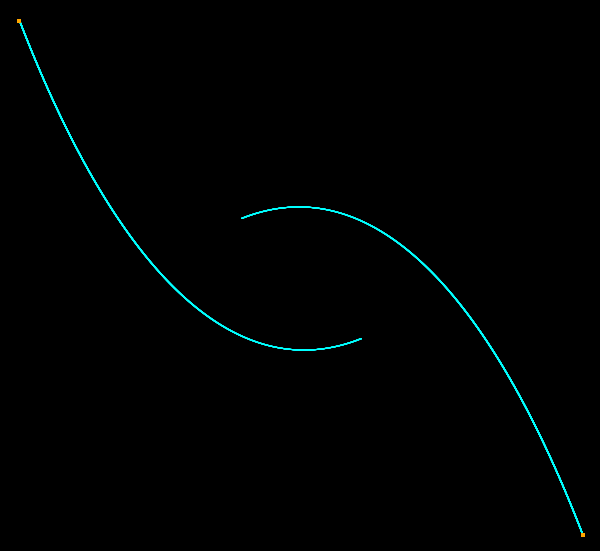
\includegraphics[width=\linewidth]{distortion3_kepler.png}
    \caption{The code \mintinline{js}{2, -3, -2, 3} is changed into \mintinline{js}{5, -2, -5, 2}}
  \end{subfigure}
  \caption{The Kepler's 2-body problem model is modified}
  \label{fig:distortion_kepler}
\end{figure}

\subsection{Adiabatic invariants}

The action variable of a periodic 1-dimensional system is an adiabatic invariant,
which does not vary when the parameters in hamiltonian change slowly \cite[p. 298]{arnold1989mathmech}\cite[p. 156]{landau1976mechanics}.

A system related to adiabatic invariance is a little difficult to imagine.
We want to use the simulator to show how adiabatic invariants work.
The codes shown below can be modified to simulate other systems related to adiabatic invariance.

Here the example adopted is the harmonic oscillator with its frequency altering slowly.
The hamiltonian is
\begin{equation*}
  \mathcal H\left(t,q,p\right)=\frac{p^2}2+\omega\left(t\right)^2\frac{q^2}2,
\end{equation*}
where $\omega\left(t\right):=4+0.05t$ changes slowly w.r.t. $t$.

By the definition of the action variable,
we can derive that the action variable for the harmonic oscillator is \cite[p. 300]{arnold1989mathmech}\cite[p. 157]{landau1976mechanics}
\begin{equation*}
  I=\frac{\mathcal H}\omega.
\end{equation*}

We are going to make the canvas draw graph for $I$ and $\mathcal H$.
Run the following codes.

\begin{minted}{js}
  // The altering parameter omega mentioned above; it should change slowly
  var omega = t => 4 + 0.05 * t;
  // The hamiltonian of the system
  var hamiltonian = (t, qp) => qp[1]**2/2 + omega(t)**2 * qp[0]**2/2;
  // Setting the hamiltonian of the system
  rungeKutta.func = canonicalEquation(1, hamiltonian);
  // There are 8 curves to be drawn on the canvas
  canvas.n = 4;
  // The labels of the curves will be q, p, H, I
  canvas.getLabelString = i => 'qpHI'[i];
  // The colors for the curves
  canvas.colors = ["white", "yellow", "pink", "blue"];
  // Tracing the H and I data when a new sample comes out
  canvas.trace = function (t, data) {
    // Calculating the hamiltonian at this time
    let h = hamiltonian(t, data);
    // To be drawn on the graph at this time: [q, p, h, h/omega]
    data = data.concat([h, h / omega(t)]);
    // Calling old method, a JavaScript trick
    return this.__proto__.trace.call(this, t, data);
  };
  // Restarting to apply the changes
  restart();
\end{minted}

The definition of the slowly altering parameter and the hamiltonian is marked with comments.
Feel free to modify them to simulate other systems with adiabatic invariants.

\begin{figure}[h]
  \centering
  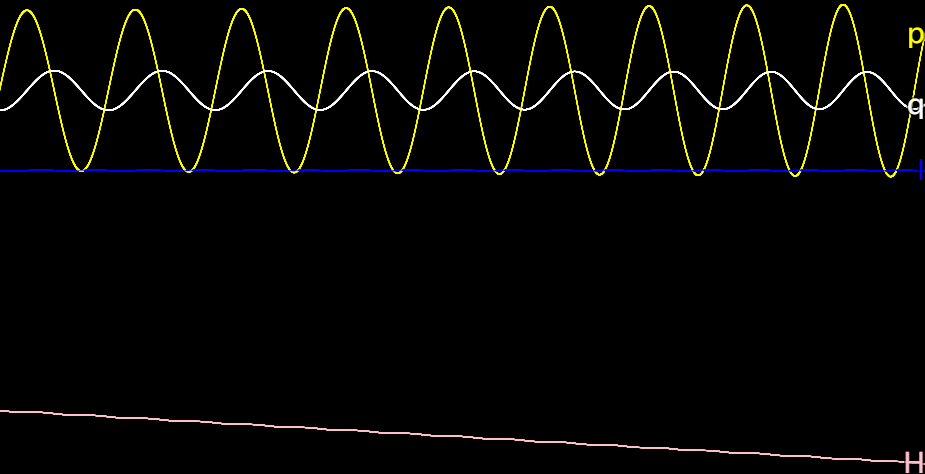
\includegraphics[width=0.6\linewidth]{adiabatic.png}
  \caption{The adiabatic invariant of a harmonic oscillator with slowly changing parameter}
  \label{fig:adiabatic}
\end{figure}

Figure \ref{fig:adiabatic} shows the result.
As can be seen, the same as theoretically predicted,
while $\omega$ and thus $\mathcal H$ changes slowly, $I$ does not vary.

\subsection{Scattered beam of particles}

Suppose there is a beam of identical particles being shot toward a central force field.
Each of the particles of the beam has hamiltonian
\begin{equation*}
  \mathcal H\left(t,q_0,q_1,p_0,p_1\right)=p_0^2+p_1^2+\frac{30}{\sqrt{q_0^2+q_1^2}}.
\end{equation*}

The beam will be scattered, and particles with different impact parameter will
have different angle of scattering \cite[p. 49]{landau1976mechanics}.
We want to study this phenomenon using the simulator.

The simulation can be done using the codes below.
Note that on low-performance devices, the simulation is slow
because there are 30 motions to be simulated at the same time.

\begin{minted}{js}
  // The total number of particles in the beam
  var n = 30;
  // The array of the n ODE solvers
  rungeKuttas = [];
  for (let i = 0; i < n; i++) {
    // Create an ODE solver
    rungeKuttas[i] = RungeKutta.solveHamiltonian(
      // Parameters list:
      2,                           // DOF
      [-20, (i - n/2)*0.3, 4, 0],  // Initial conditions
      Number.POSITIVE_INFINITY,    // Maximum time
      null,                        // Canvas; null for no canvas
      (t, qp) => {                 // The hamiltonian
        let [x, y, px, py] = qp;
        return px**2 + py**2 + 30/hypot(x,y);
      }
    );
  }

  // Create the sprite and bitmap for visualization (rpg_core.js API)
  var traceSprite = new Sprite();
  scene.addChild(traceSprite);
  traceSprite.bitmap = new Bitmap(Graphics.width, Graphics.height);

  // The scale to be used for graphing
  var my = y => 20 * y + Graphics.height/2;
  // This is the function to be called at each frame refreshing
  update = function () {
    for (let i = 0; i < n; i++) {
      // Calculate the coordinates of the point to be plotted
      let xy = [0, 1].map(j => my(rungeKuttas[i].current[j]))
      // Plotting the trajectory
      traceSprite.bitmap.setPixel(...xy, 'white');
      // Incrementing ODE solvers
      rungeKuttas[i].update();
    }
  };

  // Restarting to apply the changes
  restart();
  // Hiding the original canvas
  canvas.visible = false;
\end{minted}

\begin{figure}[h]
  \centering
  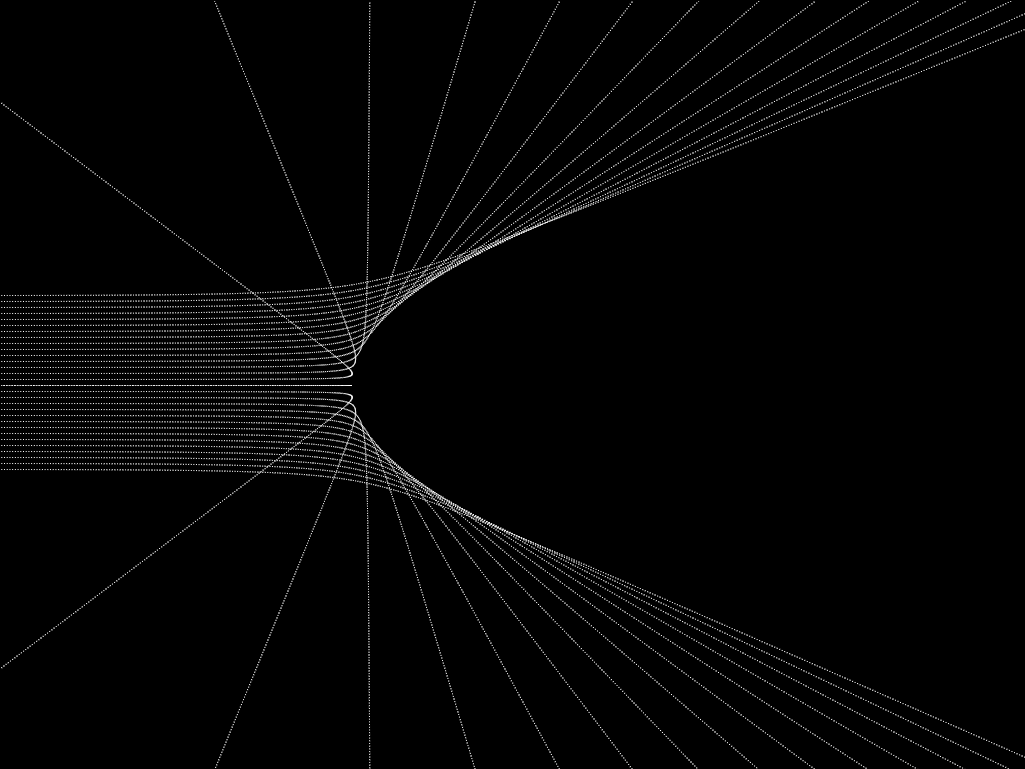
\includegraphics[width=0.8\linewidth]{scatter.png}
  \caption{The trajectories of the scattered particles}
  \label{fig:scatter}
\end{figure}

\begin{figure}[h]
  \centering
  \begin{subfigure}[b]{0.4\linewidth}
    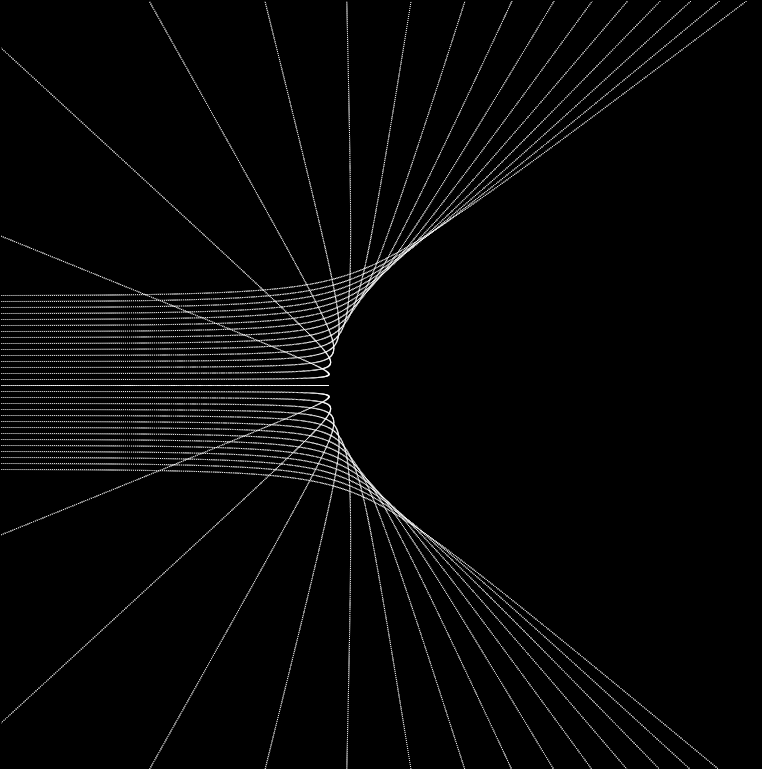
\includegraphics[width=\linewidth]{distortion_scatter.png}
    \caption{The codes \mintinline{js}{4, 0} are replaced with \mintinline{js}{3, 0}, and the curves become more bending}
  \end{subfigure}
  \begin{subfigure}[b]{0.5\linewidth}
    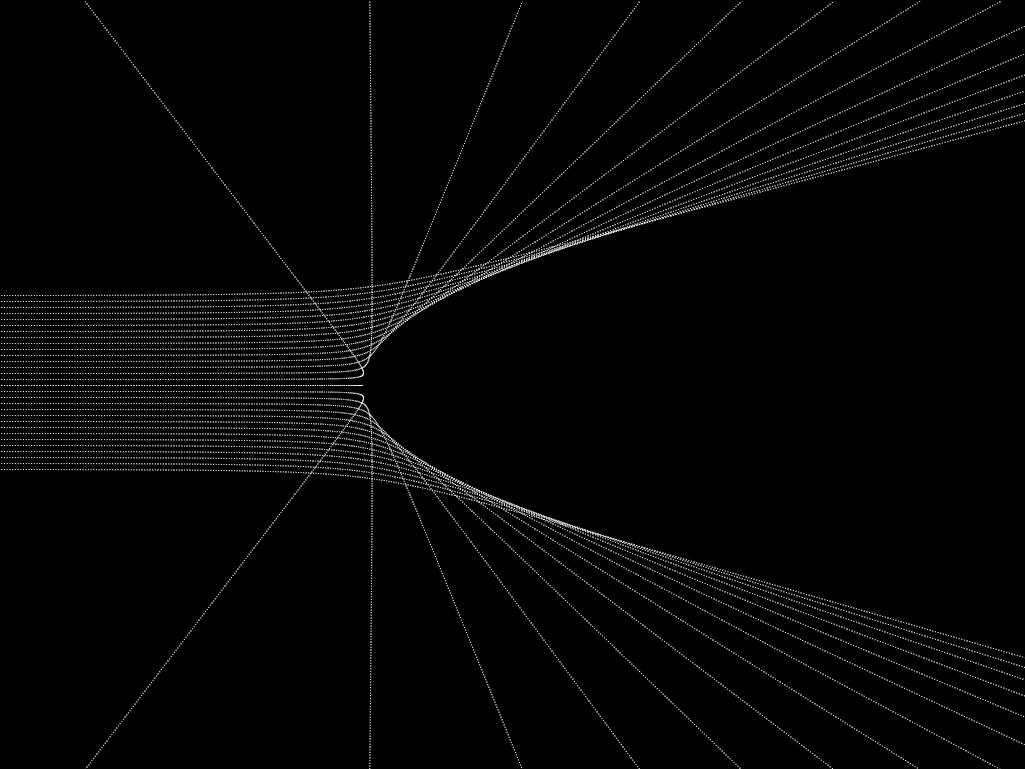
\includegraphics[width=\linewidth]{distortion2_scatter.png}
    \caption{The codes \mintinline{js}{30/hypot(x,y)} are replaced with \mintinline{js}{20/hypot(x,y)}, and the curves become less bending}
  \end{subfigure}
  \caption{The parameters of the model of scattered beam of particles is modified}
  \label{fig:distortion_scatter}
\end{figure}

The result of the codes above can be seen in Figure \ref{fig:scatter}.

The effect of scattering forms a graph rather beautiful.
It can be seen that the envelope of the trajectories of the particles
looks like a conic section, which is not thought about before we simulate it.
Then, we can be curious about what is the equation for the envelope
because it is meaningful as it indicates the safe place
where the particles will not reach.

Simple simulation like this can inspire us to study about physics.
This is exactly one of the major usages of the simulator.

One can also study how the initial velocity of the beam of the particle and the field intensity affects the trajectories.
We can use the simulator to verify that as the initial velocity decreases or the field intensity increases, the trajectories will be more bending.

The line \mintinline{js}{[-20, (i - n/2)*0.3, 4, 0],} specifies the initial conditions for the \mintinline{js}{i}th particle,
and the line \mintinline{js}{return px**2 + py**2 + 30/hypot(x,y);} specifies the hamiltonian of a particle.
We can change the codes \mintinline{js}{4, 0} into \mintinline{js}{3, 0} to make trajectories more bending,
and change the codes \mintinline{js}{30/hypot(x,y)} into \mintinline{js}{20/hypot(x,y)} to make trajectories less bending,
as can be seen in Figure \ref{fig:distortion_scatter}.

\subsection{Special relativity}

Not only classical mechanics, the simulator can simulate special relativity mechanics
because relativity mechanics can be depicted by hamiltonian mechanics.
Consider a relativity particle in a uniform gravitational field, which has hamiltonian \cite[p. 28]{landau2010fields}
\begin{equation*}
  \mathcal H\left(t,q,p\right):=\sqrt{p^2+10}-0.8q
\end{equation*}
and initial conditions $\left(q,p\right)=\left(-10,-10\right)$.

The result of the simulation is shown in Figure \ref{fig:relativity}.
The particle travels with its momentum uniformly growing,
and its speed is nearer and nearer to that of light as $t\rightarrow\infty$,
as predicted theoretically \cite[p. 24]{landau2010fields}.

\begin{figure}[h]
  \centering
  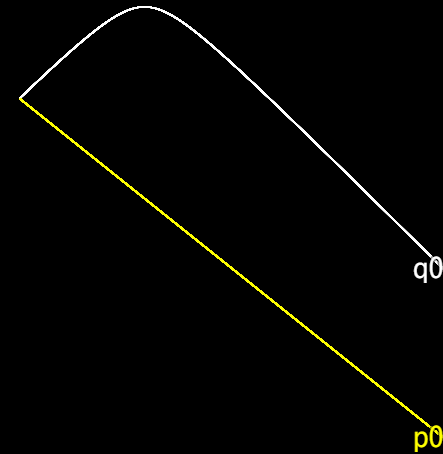
\includegraphics[width=0.25\linewidth]{relativity_gravity.png}
  \caption{The motion of a relativity particle in uniform gravity field}
  \label{fig:relativity}
\end{figure}

\section{Conclusion}

We have developed a convenient online software that can simulate hamiltonian mechanics.
There are a lot of applications that can be done with it.

The simulator is a mechanics simulator.
After the user input a hamiltonian and the initial conditions of the system,
the simulator can simulate the motion of the system,
graph the motion of it on the screen.
If a vibrating system is being simulated,
the simulator can also calculate the frequency domain of the motion using FFT after enough samples have been calculated out.

The simulator has the following advantages:
\begin{enumerate}
  \item Very small and fast.
  The simulator is rather simple but efficient.
  A user with a well-connected computer can start simulating mechanics in seconds without any preparation.

  \item Very convenient.
  Anyone with browser and Internet access can have access to the simulator without the requirement of downloading program files into the disk.
  The simulator is based on HTML and the programs is written in JavaScript which is supported by almost all browsers.

  \item Highly customizable.
  Everything of the simulator can be customized at ease.
  The simulated model, the parameters of the ODE solver, the way the simulator presents the system, etc. can all be customized.

  \item Being able to output data.
  The simulated data can be output to create mechanics datasets.
  The created datasets can be used to study the pattern of a system or be analyzed by a third-party software.

  \item Being easy to operate.
  All that the user need to do to operate the system is to write simple JavaScript codes in the console and click on the screen.
  The coding is very easy.
  If advanced usage is not needed, a user without programming experience only needs a few minutes to learn to use it.
\end{enumerate}

The simulator can be used to study motions of hamiltonian systems,
learn classical theoretical mechanics,
create animation image for presentation related to physics or online physics courses,
and create dataset of motions of a hamiltonian system.

We wrote the default model for illustrating the basic applications, mentioned in Section \ref{sec:program},
and mentioned some other examples for proposing some further applications in Section \ref{sec:examples}.

It is available on a
\href{https://UlyssesZh.github.io/rpg/mechsimul2}{webpage}.

\newpage

\bibliographystyle{abbrv}
\bibliography{mechsimul}

\newpage

\addcontentsline{toc}{section}{Acknowledgements}
\section*{Acknowledgements}

The subject is originally from my study in vibration.
I needed to write a convenient mechanics simulator to study its motion.
I want to give thanks to my instructor 李晟 (Sheng Li) because in the process,
he proposed me some ideas on the functions of the simulator
like the FFT analysis.

I want to thank my parents for their supporting me spiritually when I stuck on my study.

\end{document}
